% VUT FIT MITAI
% MSZ 2021/2022
% Author: Vladimir Dusek
% Login: xdusek27

%%%%%%%%%%%%%%%%%%%%%%%%%%%%%%%%%%%%%%%%%%%%%%%%%%%%%%%%%%%%%%%%%%%%%%%%%%%%%%%%

% Path to figures
\graphicspath{{tin/turingovy_stroje/figures}}

%%%%%%%%%%%%%%%%%%%%%%%%%%%%%%%%%%%%%%%%%%%%%%%%%%%%%%%%%%%%%%%%%%%%%%%%%%%%%%%%

\chapter{TIN~--~Turingovy stroje (jazyky přijímané TS, varianty TS, lineárně omezené automaty, vyčíslitelné funkce).}

%%%%%%%%%%%%%%%%%%%%%%%%%%%%%%%%%%%%%%%%%%%%%%%%%%%%%%%%%%%%%%%%%%%%%%%%%%%%%%%%

\section{Zdroje}

\begin{compactitem}
    \item \path{tin_2021_merged.pdf}
    \item \path{TIN_2020-10-20.mp4}
    \item \path{TIN_2020-10-27.mp4}
    \item \path{TIN_2020-11-03.mp4}
\end{compactitem}

%%%%%%%%%%%%%%%%%%%%%%%%%%%%%%%%%%%%%%%%%%%%%%%%%%%%%%%%%%%%%%%%%%%%%%%%%%%%%%%%

\section{Turingův stroj}

\begin{compactitem}
    \item Turingovy stroje jsou velmi robustní a jejich různé úpravy (determinismus, nedeterminismus, počet pásek, \dots) mají ekvivalentní vyjadřovací sílu z hlediska rozhodnutelnosti, ale z hlediska složitosti mají různou vyjadřovací sílu.

    \item Po pásce se můžeme pohybovat oběma směry. Páska je z prava nekonečná.

    \item Na TS lze nahlížet také jako na funkci, která má vstup počáteční pásku, pak nějaký výpočet (činnost TS) a jako výstup vrací stav pásky.
\end{compactitem}

\paragraph*{Definice} Turingův stroj (TS) je šestice $M = (Q, \Sigma, \Gamma, \delta, q_0, g_f)$, kde \begin{compactitem}
    \item $Q$ je konečná množina stavů;

    \item $\Sigma$ je vstupní abeceda (symboly, které se mohou vyskytovat na výchozím stavu pásky), \begin{compactitem}
        \item $\Delta \not\in \Sigma$;
    \end{compactitem}

    \item $\Gamma$ je pásková abeceda (symboly, které je možné zapisovat na pásku), \begin{compactitem}
        \item $\Sigma \subset \Gamma ~\land~ \Delta \in \Gamma ~\land~ L, R \not\in \Gamma$;
        \item Symbol $\Delta$ značí tzv. blank (prázdný symbol), který se vyskytuje na místech pásky,
        která nebyla ještě použita (může ale být na pásku zapsán i později).
    \end{compactitem}

    \item $\delta$ je přechodová funkce (parciální funkce), \begin{compactitem}
        \item $\delta : (Q - \{ q_f \}) \times \Gamma \rightarrow Q \times (\Gamma \cup \{ L, R \})$;
    \end{compactitem}

    \item $q_0$ je výchozí stav, \begin{compactitem}
        \item $q_0 \in Q$;
    \end{compactitem}

    \item $q_f$ je koncový stav, \begin{compactitem}
        \item $q_f \in Q$;
    \end{compactitem}
\end{compactitem}

\paragraph*{Konfigurace} Konfigurace TS je trojice $(q, \alpha, n) \in Q \times \{ \gamma \Delta^{\omega} ~|~ \gamma \in \Gamma \} \times \mathbb{N}$, kde \begin{compactitem}
    \item $q$ je aktuální stav;
    \item $\alpha$ značí stav pásky;
    \item $n$ značí pozici hlavy.
\end{compactitem}

\paragraph*{Počáteční konfigurace} Počáteční konfigurace je taková konfigurace $(q_0, \gamma \Delta^{\omega}, 0)$, kde $\gamma \Delta^{\omega}$ je výchozí stav pásky a $q_0$ je výchozí stav.

\paragraph*{Koncová konfigurace} Koncová konfigurace je taková konfigurace $(q_f, \gamma \Delta^{\omega}, n)$, kde $\gamma \Delta^{\omega}$ je stav pásky a $q_f$ je koncový stav.

\paragraph*{Přechod} Přechod (krok výpočtu) TS $M$ definujeme jako nejmenší binární relaci $\vdash$ takovou, že $\forall q_1, q_2 \in Q ~ \forall \gamma \in \Gamma^{\omega} ~ \forall n \in \mathbb{N} ~ \forall b \in \Gamma$: \begin{compactitem}
    \item $(q_1, \gamma, n) \vdash (q_2, \gamma, n + 1)$ pro $\delta(q_1, \gamma_n) = (q_2, R)$ -- operace posunu hlavy doprava při $\gamma_n$ po hlavou;

    \item $(q_1, \gamma, n) \vdash (q_2, \gamma, n - 1)$ pro $\delta(q_1, \gamma_n) = (q_2, L)$ -- operace posunu hlavy doleva při $\gamma_n$ po hlavou;

    \item $(q_1, \gamma, n) \vdash (q_2, s_b^n(\gamma), n + 1)$ pro $\delta(q_1, \gamma_n) = (q_2, b)$ -- operace zápisu symbolu $b$ při $\gamma_n$ po hlavou.
\end{compactitem}

Pro libovolný řetězec $\gamma \in \Gamma^{\omega}$ a číslo $n \in \mathbb{N}$ označme $\gamma_n$ n-tý symbol daného řetězce a označme $s_n^b(\gamma)$ řetězec, který vznikne z $\gamma$ záměnou $\gamma_n$ za $b$.

\paragraph*{Jazyk přijímaný} \begin{compactitem}
    \item Řetězec $w \in \Sigma^*$ je přijat TS $M = (Q, \Sigma, \Gamma, \delta, q_0, g_f)$, jesliže pro $M$ platí:\break $(q_0, \Delta \gamma \Delta^{\omega}, 0) \vdash^* (q_f, \gamma', n)$ pro nějaké $\gamma, \gamma' \in \Gamma^*$ a $n \in \mathbb{N}$.

    \item Množinu $L(M) = \{ w ~|~ w \text{ je přijat TS } M \} \subseteq \Sigma^*$ nazýváme jazyk přijímaný TS $M$.
\end{compactitem}

\begin{figure}[H]
    \centering
    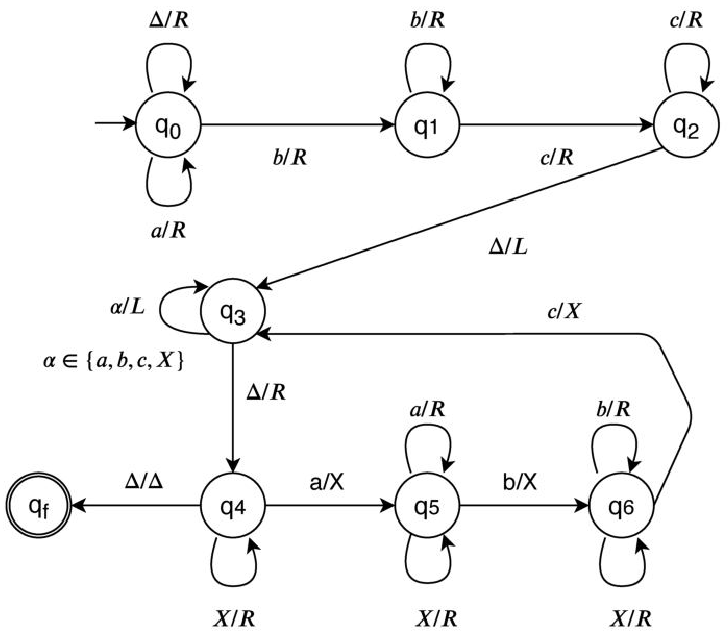
\includegraphics[width=0.8\linewidth]{ts_example.pdf}
    \caption{Příklad TS, který přijímá jazyk $L = \{ a^n b^n c^n ~|~ n > 0 \}$.}
\end{figure}

\paragraph*{Univerzální turingův stroj} Je možné sestrojit takový turingův stroj, který má vlastnost, že dokáže simulovat chování jiného Turingova stroje. Může fungovat jako interpret. Na vstupu přijme zakódovaný Turingův stroj (program) a vstup, který vykoná.

%%%%%%%%%%%%%%%%%%%%%%%%%%%%%%%%%%%%%%%%%%%%%%%%%%%%%%%%%%%%%%%%%%%%%%%%%%%%%%%%

\section{Varianty turingova stroje}

\subsection{Deterministický turingův stroj} Deterministický turingův stroj (DTS) je výchozí turingův stroj (DTS = TS).

\subsection{Vícepáskový turingův stroj}

Vícepáskový TS má stejnou (rozhodovací) vyjadřovací sílu jako jednopáskový TS (jsou mezi sebou převoditelné). Formálně to znamená, že pro každý $k$-páskový TS $M$ existuje jednopáskový TS $M'$ takový, že $L(M) = L(M')$. Myšlenka důkazu spočívá v tom, že $k$ pásek můžeme simulovat jednou. Jeden symbol na pásce potom bude mít formu $2k$-tice. Pro každou pásku jsou potřeba 2 prvky v n-tici, protože v jedné je třeba si udržovat pozici hlavy. Myšlenka je na obrázku.

\begin{figure}[H]
    \centering
    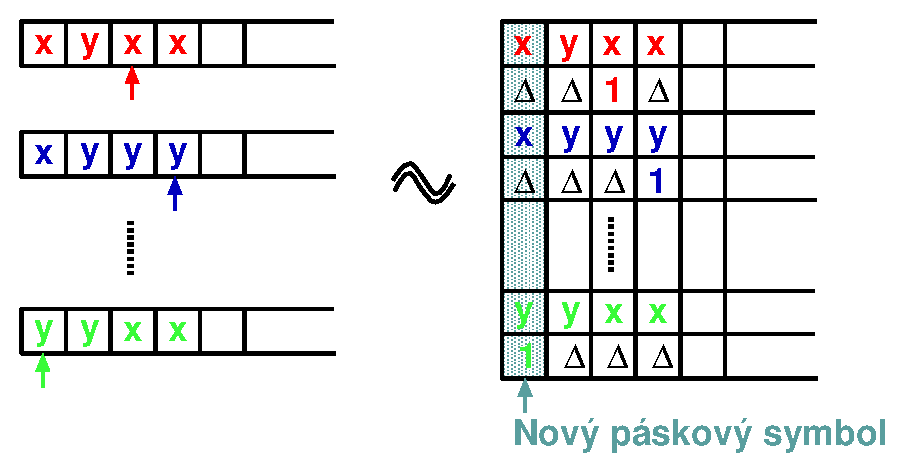
\includegraphics[width=1\linewidth]{ts_vicepaskovy_dukaz.pdf}
    \caption{Myšlenka převodu vícepáskového TS na jednopáskový.}
\end{figure}

\paragraph*{Definice} Vícepáskový TS se od TS liší tvarem přechodové funkce, disponuje více páskami a s každou může pracovat zároveň. Formálně:

\begin{compactitem}
    \item $\delta$ je přechodová funkce (parciální funkce). $$\delta : (Q - \{ q_f \} ) \times \Gamma_1 \times \ldots \times \Gamma_n \rightarrow Q \times ( \Gamma_1 \cup \{ L, R \} ) \times \ldots \times ( \Gamma_n \cup \{ L, R \} )$$
\end{compactitem}

\paragraph*{Příklad} Příklad vícepáskového TS.

\begin{figure}[H]
    \centering
    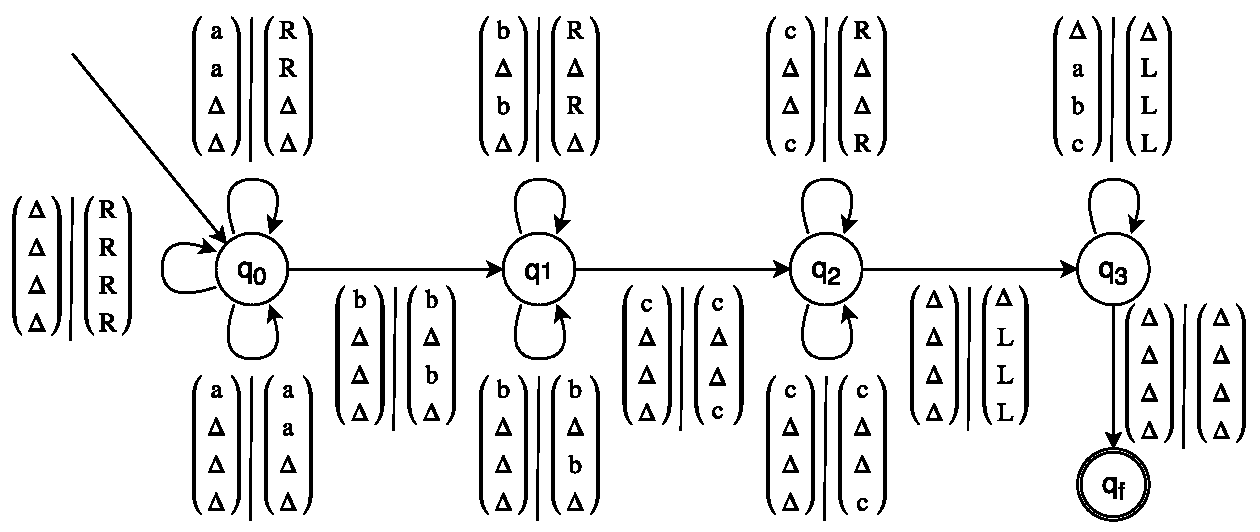
\includegraphics[width=1\linewidth]{ts_vicepaskovy_example.pdf}
    \caption{Příklad 4-páskový TS, který přijímá jazyk $L = \{ a^n b^n c^n ~|~ n > 0 \}$.}
\end{figure}

\subsection{Nedeterministický turingův stroj}

Nedeterministický TS (NTS) má stejnou (rozhodovací) vyjadřovací sílu jako DTS (jsou mezi sebou převoditelné). Formálně to znamená, že pro každý NTS $M$ existuje DTS $M'$ takový, že $L(M) = L(M')$. Myšlenka důkazu spočívá v tom, že strom běhů NTS prohledáváme do šířky (jelikož běh může obsahovat smyčky). Konkrétně, NTS $M$ budeme simulovat třípáskovým DTS. Význam jednotlivých pásek tohoto
stroje je následující: \begin{compactitem}
    \item Páska 1 obsahuje vstupní řetězec.
    \item Páska 2 je pracovní páska. Obsahuje kopii pásky 1 ohraničenou vhodnými speciálními značkami. Po neúspěšném pokusu o přijetí je její obsah smazán a obnoven z první pásky.
    \item Páska 3 obsahuje kódovanou volbu posloupností přechodů; při neúspěchu bude její obsah nahrazen jinou posloupností.
\end{compactitem}

\paragraph*{Definice} NTS se od TS liší tvarem přechodové funkce. Formálně:

\begin{compactitem}
    \item $\delta$ je přechodová funkce (parciální funkce). $$\delta : (Q - \{ q_f \}) \times \Gamma \rightarrow 2^{Q \times (\Gamma \cup \{ L, R \})}$$
\end{compactitem}

\paragraph*{Příklad} Příklad nedeterministického TS, kde nedeterminismus může přinést značné zjednodušení, je TS, který přijímá jazyk $L = \{ ww ~|~ w \in \Sigma^* \}$.

\subsection{Úplný turingův stroj}

Úplný turingův stroj je takový TS, který pro libovolný vstup zastaví, a buď přijme nebo odmítne (nemůže se zacyklit). Úplné turingovy stroje mají menší (rozhodovací) vyjadřovací sílu než obecný turingův stroj. Nedeterministický Turingův stroj je úplný, právě když pro každý vstup je každá výpočetní větev konečná (tj. pro každý vstup vždy zastaví).

\begin{compactitem}
    \item Jazyk $L \subseteq \Sigma^*$ se nazývá: \begin{compactitem}
        \item Rekurzivně vyčíslitelný ($REL, \mathcal{L}_0, \mathcal{L}_{RE}$), jestliže $L = L(M)$ pro nějaký TS $M$.

        \item Rekurzivní ($RL, \mathcal{L}_{Rec}$), jestliže $L = L(M)$ pro nějaký úplný TS $M$.
    \end{compactitem}

    \item Je-li $M$ úplný TS, pak říkáme, že $M$ rozhoduje jazyk $L(M)$.

    \item Ke každému rekurzívnímu jazyku existuje TS, který ho rozhoduje, tj. zastaví pro každé vstupní slovo (např. na pásku zapíše $YES$ nebo $NO$).

    \item TS přijímající rekurzívně vyčíslitelný jazyk $L$ zastaví pro každé $w \in L$, ovšem pro $w \not\in L$ může zastavit, ale také může donekonečna cyklit.

    \item Platí $2^{\Sigma^*} \subset \mathcal{L}_{RE} \subset \mathcal{L}_{Rec} \subset \mathcal{L}_1$.
\end{compactitem}

%%%%%%%%%%%%%%%%%%%%%%%%%%%%%%%%%%%%%%%%%%%%%%%%%%%%%%%%%%%%%%%%%%%%%%%%%%%%%%%%

\section{Lineárně omezený automat}

\begin{compactitem}
    \item Lineárně omezený automat (LOA) je nedeterministický TS, který nikdy neopustí tu část pásky, na níž je zapsán jeho vstup. \begin{compactitem}
        \item Takový turingův stroj, který má lineárně omezenou velikost pásky vůči délce vstupu (\textit{Linear Bounded Automata}). Avšak, díky možnosti zápisu n-tic na pásku (viz důkaz u vícepaskových TS), je možné pásku zkomprimovat tak, že stačí pouze tolik místa, kolik je délka vstupního slova.
    \end{compactitem}

    \item Deterministický LOA můžeme definovat jako DTS, který nikdy neopustí část pásky se zapsaným vstupem. \begin{compactitem}
        \item Není známo, zda deterministický LOA je či není striktně slabší než LOA.
    \end{compactitem}

    \item Třída jazyků, kterou lze generovat kontextovými gramatikami, odpovídá třídě jazyků, které lze přijímat LOA.

    \item Z konečné délky pásky vyplývá, že pro každý LOA existuje pouze konečné množství konfigurací. To znamená, že pokud LOA cyklí, jsme to schopni detekovat. A tedy, problémy pro LOA jsou rozhodnutelné.
\end{compactitem}

% \item Jazyky $L_1$ jsou příjímány lineárně omezeným automatem -- nedeterministický turingův stroj (NTS) s lineárně omezenou páskou. \begin{compactitem}
%     \item Omezení lineární funkcí v závislosti na délce vstupního řetězce.
%     \item Z toho vyplývá, že řetězec se nemůže zkracovat, ledaže se derivuje $S \Rightarrow \epsilon$, ale v takovém případě se S nemůže vyskytovat na pravé straně žádného pravidla.
%     \item Formálně: pokud $\alpha \Rightarrow \beta$, pak $|\alpha| \leq |\beta|$ (s vyjímkou $S \Rightarrow \epsilon$).

%%%%%%%%%%%%%%%%%%%%%%%%%%%%%%%%%%%%%%%%%%%%%%%%%%%%%%%%%%%%%%%%%%%%%%%%%%%%%%%%

\section{Vyčíslitelné funkce}

\todo{todo}
